\documentclass[11pt]{article}
\usepackage{appendix}
\usepackage{graphicx} 
\usepackage{setspace}
\usepackage{amsmath,float,verbatim,multicol}
\usepackage{array}
\usepackage{lscape}
\usepackage{hyperref}

\usepackage{amssymb}
\bibliographystyle{plainnat}
\usepackage[round]{natbib}
\usepackage{multirow}

\setlength{\textheight}{8.8in} \setlength{\textwidth}{6.3in}
\setlength{\oddsidemargin}{0.2in} \setlength{\topmargin}{-0.30in}
\setlength{\footnotesep}{10.0pt}

\newcommand{\ol}{\overline}



\renewcommand{\baselinestretch}{1.25}
\title{Solving an Stochastic Infinitely-Lived Human Capital Accumulation Problem}
\author{ Trevor Gallen \\ Econ 64200 }
\date{Fall 2023}

\begin{document}
\bibliographystyle{myplainnat}
%\bibpunct{(}{)}{;}{a}{}{,}6868

\maketitle

This homework is the first part of a multi-part homework.  This homework takes the deterministic model we had in the first homework and adds (1) a stochastic state variable and (2) a second dimension of choice, and asks you to solve it in Matlab.\\

\textbf{Deliverables}
\begin{itemize}
\item You should have a word/\LaTeX document that has three sections: 
\begin{enumerate}
\item Discusses the model and answers the questions I pose throughout.
\item Contains the tables and figures you will produce.
\item Contains a discussion of your programming choices if you had to make any.
\end{enumerate}
\item You should have a Matlab file or set of files (zipped) that contain \textbf{all} your programs and raw data.  There should be a file called ``Main.M" that produces everything I need in one click.
\end{itemize}


\section{Model}
Infinitely-lived households start each period with human capital endowment $h_t$, and have period utility over consumption $c_t$.  They have one unit of time each period, which they use to either study $i_t$ or work $L_t$ . If they study, their human capital for next period grows subject to a stochastic productivity rate $A_t$ known at time $t$, while if they work, consumption increases.  Households have access to a savings technology which pays interest rate $1+r$ when they save $w_t$.  They maximize the net present value of utility discounted at a rate $0<\beta<1$:
$$\sum_{t=0}^\infty \log(c_t)$$
subject to the law of motion of human capital:
$$h_{t+1}=(1-\delta)h_t+exp(A_t)i_t^\gamma$$
Their budget constraint:
$$c_t+w_t=h_tL_t+(1+r)w_{t-1}$$
And the law of motion for human capital accumulation $A_t$:
$$A_{t+1}=\rho A_t+\epsilon_t$$
$$\epsilon_t\sim \mathcal{N}\left(0,\sigma^2_\epsilon\right)$$

\section{Basic Matlab}
Now, let the following numerical assumptions hold:
\begin{table}[ht!]
\centering
\begin{tabular}{lcc}
\hline
\hline
\multicolumn{3}{c}{Table 1: Calibration}\\
\hline
Concept & Parameter & Value \\ 
Discount factor & $\beta$ & 0.95\\
Ability to accumulate human capital: &  $A$ & 1\\
Human capital depreciation rate:&  $\delta$  & 0.05\\
Decreasing returns to human capital investment: & $\gamma$  & 0.6\\
AR(1) parameter for productivity shocks: & $\rho$  & 0.95\\
Variance of productivity shocks: &  $\sigma^2_\epsilon$  & 0.01\\
Interest rate: &  $r$  & $\frac{1}{0.95}-1$\\
\hline
\hline
\end{tabular}
\end{table}

\textbf{Question 2:} Write a Matlab program that takes in the parameterization of Table 1 and uses value function iteration to solve the agent's problem.  To be clear, your problem is now $V(h_t,A_t,w_{t-1})$, and has a choice over not just $i_t$ but also $w_t$.  Also note that you will have to truncate the distribution of $A_{t+1}$:  be clear about your justification for what you choose!\footnote{I suggest bounding state variable $h\in\left[7.5,10\right]$, $w\in\left[0 , 1.5\right]$, and finding your own bounds for $A$.  Moreover, I suggest taking only five points in each space to start (125 points total), so that you ``fail quickly" if something isn't working.  }\\
\ \\
\textbf{See Main.m for code.}\\
\ \\

\begin{figure}[ht!]
\centering
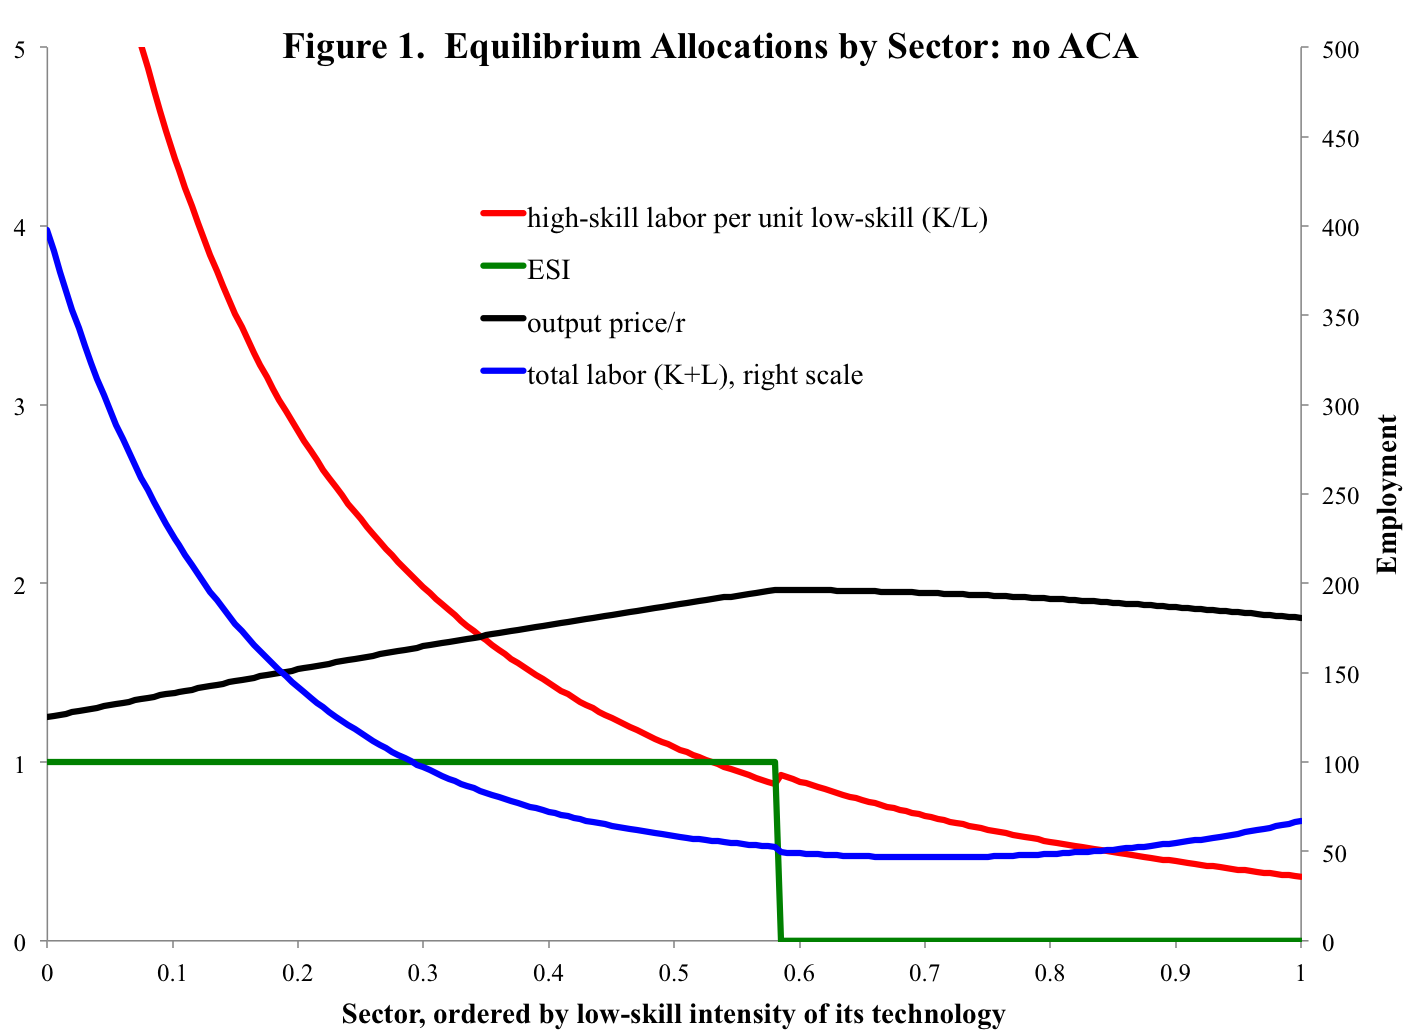
\includegraphics[scale=0.5]{Fig1.png}
\caption{My code uses both Policy Function Iteration and Value Function Iteration.  This figure compares the speed of the two, plotting on the x-axis seconds of run-time and on the y-axis the error between value function updates (when solving the actual value function).  It omits the value function changes that do not involve maximization, to compare apples to apples.  What a speed difference!}
\end{figure}





\textbf{Question 3:} Plot the two-dimensional policy functions for $i$ and for $s$ as a function of $A$ and $w$ when $h=8.46$.  \\
\ \\
\begin{figure}[ht!]
\centering
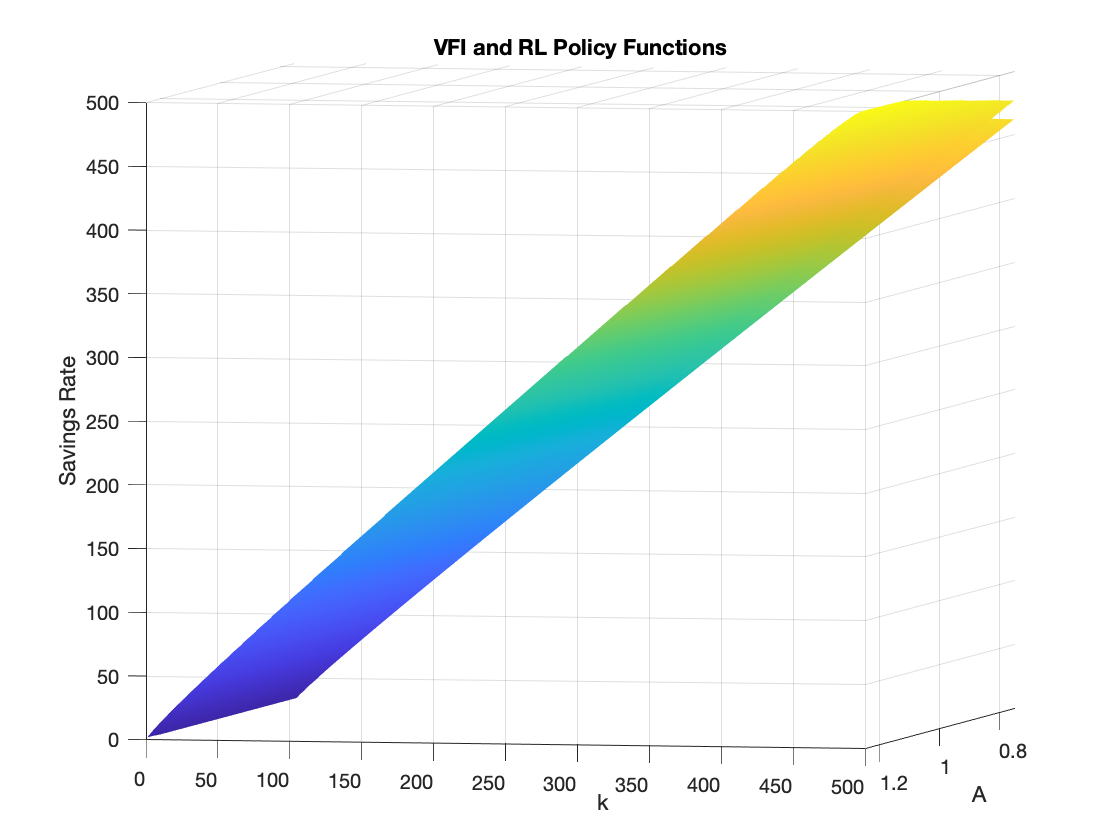
\includegraphics[scale=0.5]{Fig2.png}
\caption{This figure plots the policy function for $i^*(s,A|h=8.46)$.}
\end{figure}

\begin{figure}[ht!]
\centering
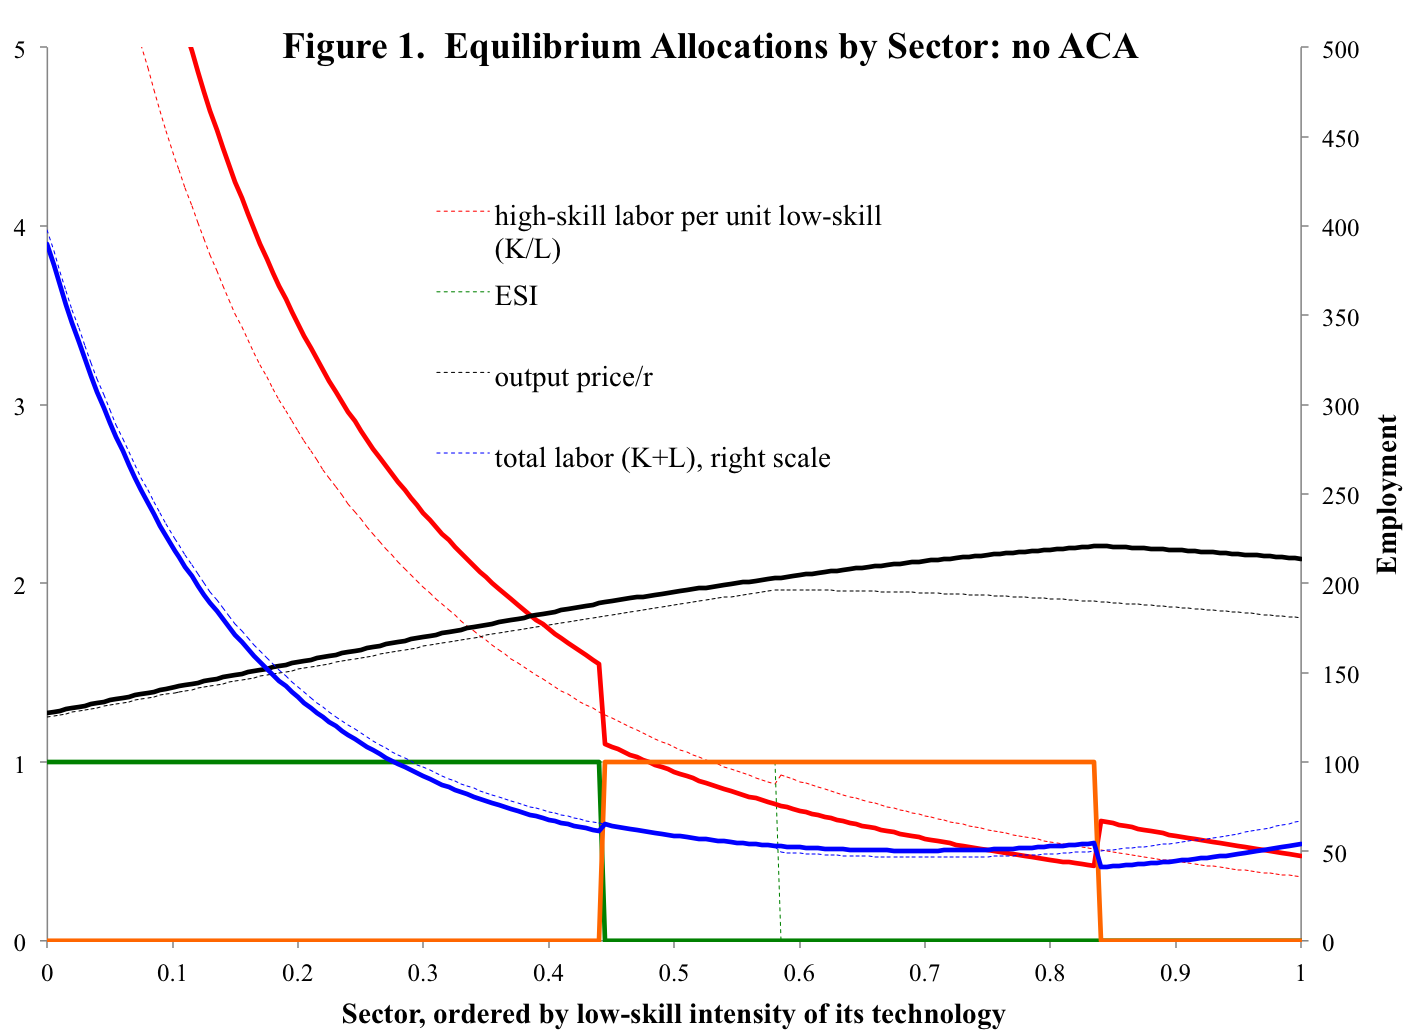
\includegraphics[scale=0.5]{Fig3.png}
\caption{This figure plots the policy function for $s^*(s,A|h=8.46)$.}
\end{figure}

\begin{figure}[ht!]
\centering
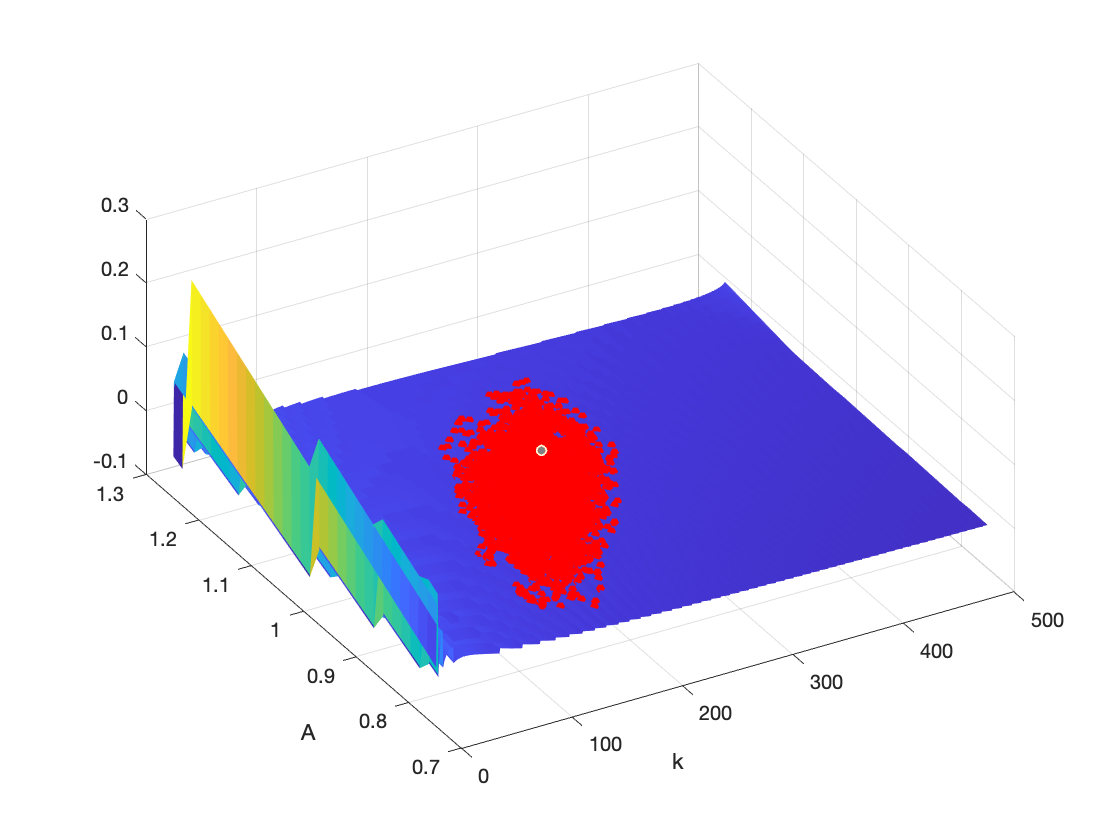
\includegraphics[scale=0.5]{Fig4.png}
\caption{This figure plots the value function for $s^*(s,A|h=8.46)$.}
\end{figure}


\textbf{Question 4:} Assuming the productivity parameter is independently drawn across individuals, use your estimated policy functions for $i$ and $s$, as well as the law of motion of $A$ to simulate the savings over many periods, so your initialization doesn't matter for at least 1000 individuals.  Using your simulated individuals, plot the stationary distribution of wealth in this society.

\begin{figure}[ht!]
\centering
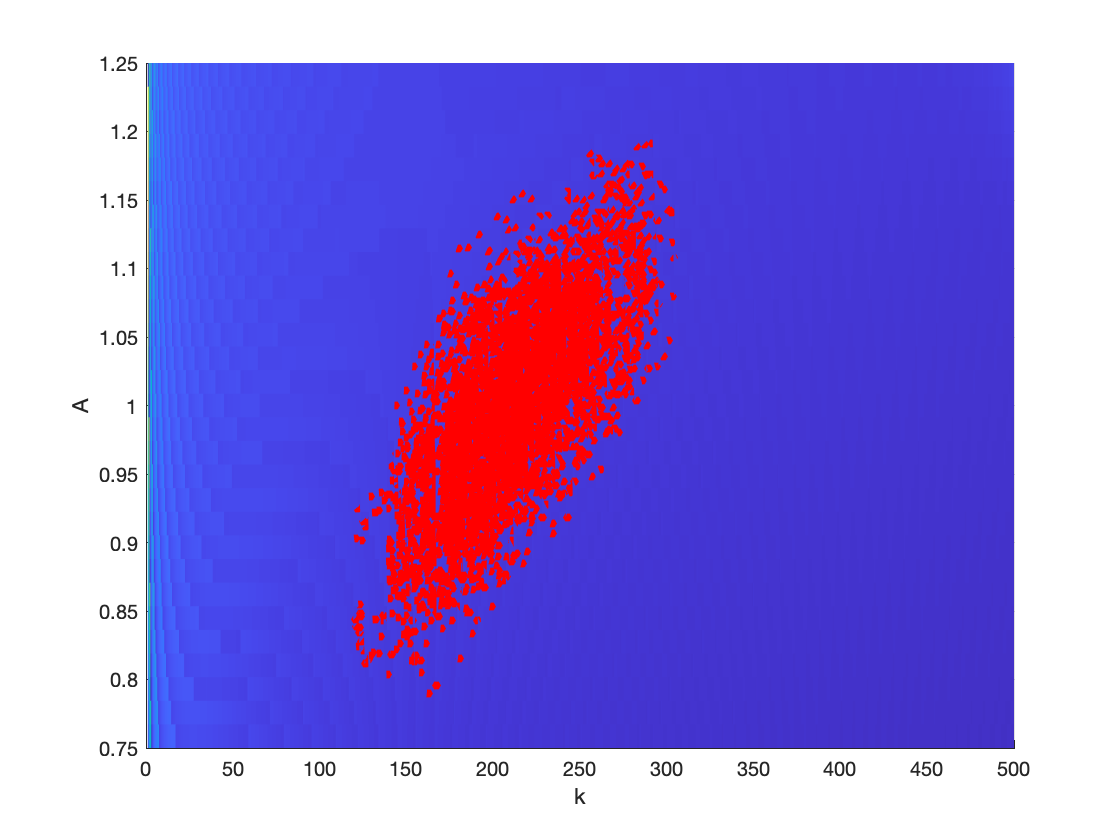
\includegraphics[scale=0.5]{Fig5.png}
\caption{This figure plots the stationary wealth distribution.}
\end{figure}



\end{document}





